190. \begin{figure}[ht!]
\center{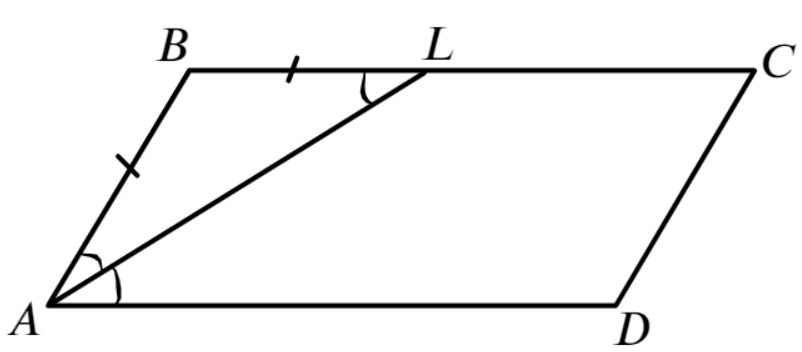
\includegraphics[scale=0.35]{g8-189.png}}
\end{figure}\\
Углы $BAL$ и $LAD$ равны, так как $BL$ --- биссектриса угла $A,$ а углы $BLA$ и $LAD$ равны как накрест лежащие, значит $\angle BAL=\angle BLA$ и треугольник $BAL$ является равнобедренным, $BA=BL.$ Так как $BL:LC=2:1,$ получаем соотношение $BC=1,5AB.$ При этом $(AB+BC)\cdot2=100$см, откуда $2,5AB=50,\ AB=20$см, $BC=30$см.\\
